

\tikzset{every picture/.style={line width=0.75pt}} %set default line width to 0.75pt        
\begin{center}
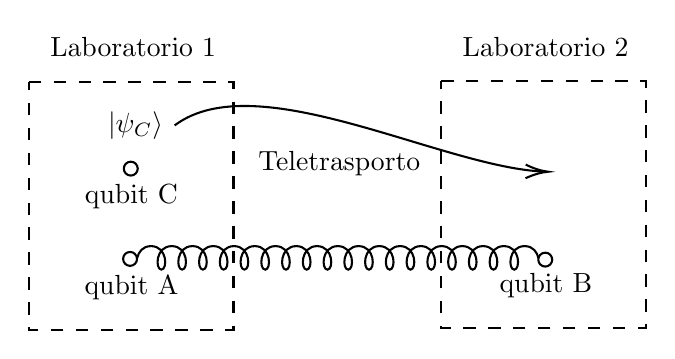
\begin{tikzpicture}[x=0.75pt,y=0.75pt,yscale=-1,xscale=1]
%uncomment if require: \path (0,300); %set diagram left start at 0, and has height of 300

%Shape: Rectangle [id:dp019828091081898647] 
\draw  [dash pattern={on 4.5pt off 4.5pt}] (101,91.17) -- (199.67,91.17) -- (199.67,210.5) -- (101,210.5) -- cycle ;
%Shape: Rectangle [id:dp7316415823282396] 
\draw  [dash pattern={on 4.5pt off 4.5pt}] (299.67,90.5) -- (398.33,90.5) -- (398.33,209.83) -- (299.67,209.83) -- cycle ;
%Shape: Spring [id:dp4458037239709285] 
\draw   (153.29,175.83) .. controls (153.92,173) and (155.92,170.17) .. (159.92,170.17) .. controls (167.92,170.17) and (167.92,181.5) .. (164.92,181.5) .. controls (161.92,181.5) and (161.92,170.17) .. (169.92,170.17) .. controls (177.92,170.17) and (177.92,181.5) .. (174.92,181.5) .. controls (171.92,181.5) and (171.92,170.17) .. (179.92,170.17) .. controls (187.92,170.17) and (187.92,181.5) .. (184.92,181.5) .. controls (181.92,181.5) and (181.92,170.17) .. (189.92,170.17) .. controls (197.92,170.17) and (197.92,181.5) .. (194.92,181.5) .. controls (191.92,181.5) and (191.92,170.17) .. (199.92,170.17) .. controls (207.92,170.17) and (207.92,181.5) .. (204.92,181.5) .. controls (201.92,181.5) and (201.92,170.17) .. (209.92,170.17) .. controls (217.92,170.17) and (217.92,181.5) .. (214.92,181.5) .. controls (211.92,181.5) and (211.92,170.17) .. (219.92,170.17) .. controls (227.92,170.17) and (227.92,181.5) .. (224.92,181.5) .. controls (221.92,181.5) and (221.92,170.17) .. (229.92,170.17) .. controls (237.92,170.17) and (237.92,181.5) .. (234.92,181.5) .. controls (231.92,181.5) and (231.92,170.17) .. (239.92,170.17) .. controls (247.92,170.17) and (247.92,181.5) .. (244.92,181.5) .. controls (241.92,181.5) and (241.92,170.17) .. (249.92,170.17) .. controls (257.92,170.17) and (257.92,181.5) .. (254.92,181.5) .. controls (251.92,181.5) and (251.92,170.17) .. (259.92,170.17) .. controls (267.92,170.17) and (267.92,181.5) .. (264.92,181.5) .. controls (261.92,181.5) and (261.92,170.17) .. (269.92,170.17) .. controls (277.92,170.17) and (277.92,181.5) .. (274.92,181.5) .. controls (271.92,181.5) and (271.92,170.17) .. (279.92,170.17) .. controls (287.92,170.17) and (287.92,181.5) .. (284.92,181.5) .. controls (281.92,181.5) and (281.92,170.17) .. (289.92,170.17) .. controls (297.92,170.17) and (297.92,181.5) .. (294.92,181.5) .. controls (291.92,181.5) and (291.92,170.17) .. (299.92,170.17) .. controls (307.92,170.17) and (307.92,181.5) .. (304.92,181.5) .. controls (301.92,181.5) and (301.92,170.17) .. (309.92,170.17) .. controls (317.92,170.17) and (317.92,181.5) .. (314.92,181.5) .. controls (311.92,181.5) and (311.92,170.17) .. (319.92,170.17) .. controls (327.92,170.17) and (327.92,181.5) .. (324.92,181.5) .. controls (321.92,181.5) and (321.92,170.17) .. (329.92,170.17) .. controls (337.92,170.17) and (337.92,181.5) .. (334.92,181.5) .. controls (331.92,181.5) and (331.92,170.17) .. (339.92,170.17) .. controls (344,170.17) and (346,173.12) .. (346.58,176.01) ;
%Straight Lines [id:da8152639809390969] 
\draw    (149.83,176.33) ;

\draw [shift={(149.83,176.33)}, rotate = 0] [color={rgb, 255:red, 0; green, 0; blue, 0 }  ][line width=0.75]      (0, 0) circle [x radius= 3.35, y radius= 3.35]   ;
%Straight Lines [id:da6744702488611394] 
\draw    (150.17,132.83) ;

\draw [shift={(150.17,132.83)}, rotate = 0] [color={rgb, 255:red, 0; green, 0; blue, 0 }  ][line width=0.75]      (0, 0) circle [x radius= 3.35, y radius= 3.35]   ;
%Straight Lines [id:da8857801521218736] 
\draw    (349.87,176.67) ;

\draw [shift={(349.87,176.67)}, rotate = 0] [color={rgb, 255:red, 0; green, 0; blue, 0 }  ][line width=0.75]      (0, 0) circle [x radius= 3.35, y radius= 3.35]   ;
%Curve Lines [id:da07911679295346907] 
\draw    (171.33,112) .. controls (210.93,82.3) and (300.85,132.64) .. (349.86,134.3) ;
\draw [shift={(351.33,134.33)}, rotate = 180.78] [color={rgb, 255:red, 0; green, 0; blue, 0 }  ][line width=0.75]    (10.93,-3.29) .. controls (6.95,-1.4) and (3.31,-0.3) .. (0,0) .. controls (3.31,0.3) and (6.95,1.4) .. (10.93,3.29)   ;


% Text Node
\draw (151.33,74) node  [align=left] {Laboratorio 1};
% Text Node
\draw (350,74) node  [align=left] {Laboratorio 2};
% Text Node
\draw (150.5,190) node  [align=left] {qubit A};
% Text Node
\draw (150.5,146.5) node  [align=left] {qubit C};
% Text Node
\draw (152.5,112) node   {$|\psi _{C} \rangle $};
% Text Node
\draw (350.2,189) node  [align=left] {qubit B};
% Text Node
\draw (250.67,130.33) node  [align=left] {Teletrasporto};


\end{tikzpicture}
\end{center}